%%%%%%%%%%%%%%%%%%%%%%%%%%%%%%%
%   Figures for chapter 1
%%%%%%%%%%%%%%%%%%%%%%%%%%%%%%%

\newcommand{\figDrlLocomotionMotivation}{
    \begin{figure}[!ht]
        \centering
        \begin{subfigure}[b]{0.45\textwidth}
            \centering
            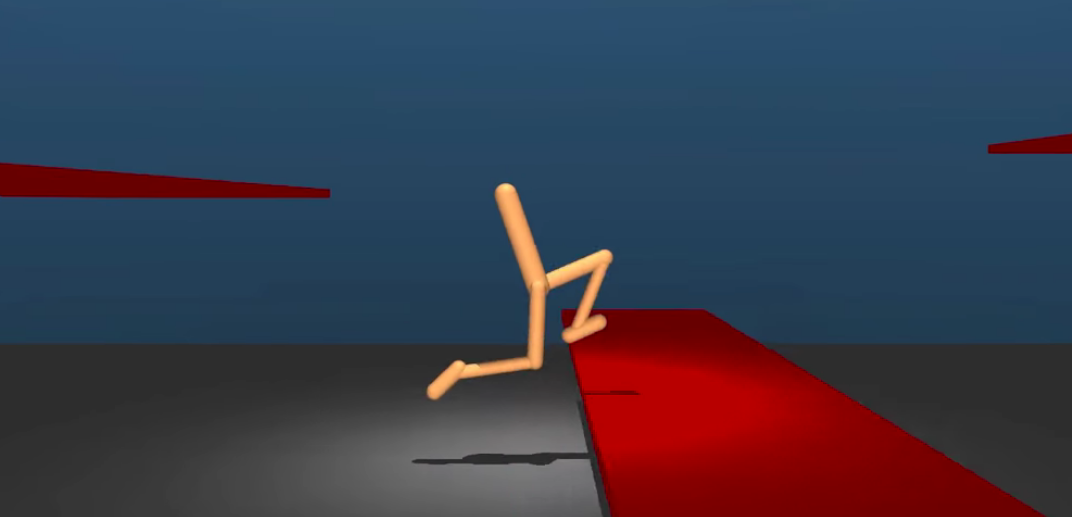
\includegraphics[width=0.9\textwidth]{./chapters/chapter_1/imgs/img_ch1_emergence_of_locomotion.png}
            \caption{}
            \label{fig:ch1_emergence_locomotion}
        \end{subfigure}
        \begin{subfigure}[b]{0.45\textwidth}
            \centering
            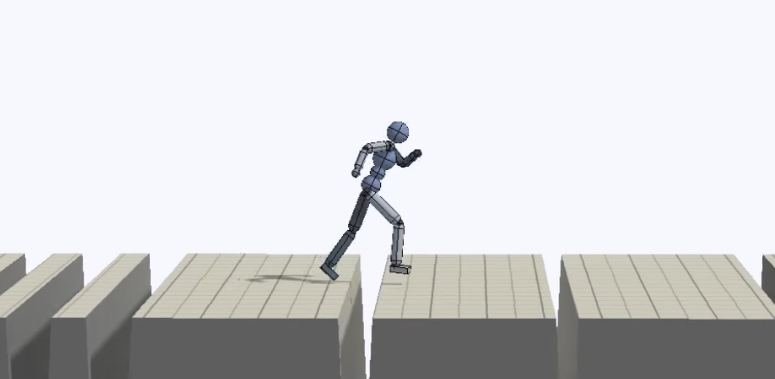
\includegraphics[width=0.9\textwidth]{./chapters/chapter_1/imgs/img_ch1_deepmimic.png}
            \caption{}
            \label{fig:ch1_deepmimic}
        \end{subfigure}
        \caption{Some results from applying Deep Reinforcement Learning to locomotion. 
                    a) Biped traversing simulated environment \citep{DeepmindEmergenceLocomotion}.
                    b) Humanoid traversing simulated environment \citep{DeepMimic} }
        \label{fig:ch1_motivation_drl_locomotion}
    \end{figure}
}

\newcommand{\figDrlBenchmarks}{
    \begin{figure}
        %% Controlsuite
        \centering
        \begin{subfigure}[b]{1.0\textwidth}
            \centering
            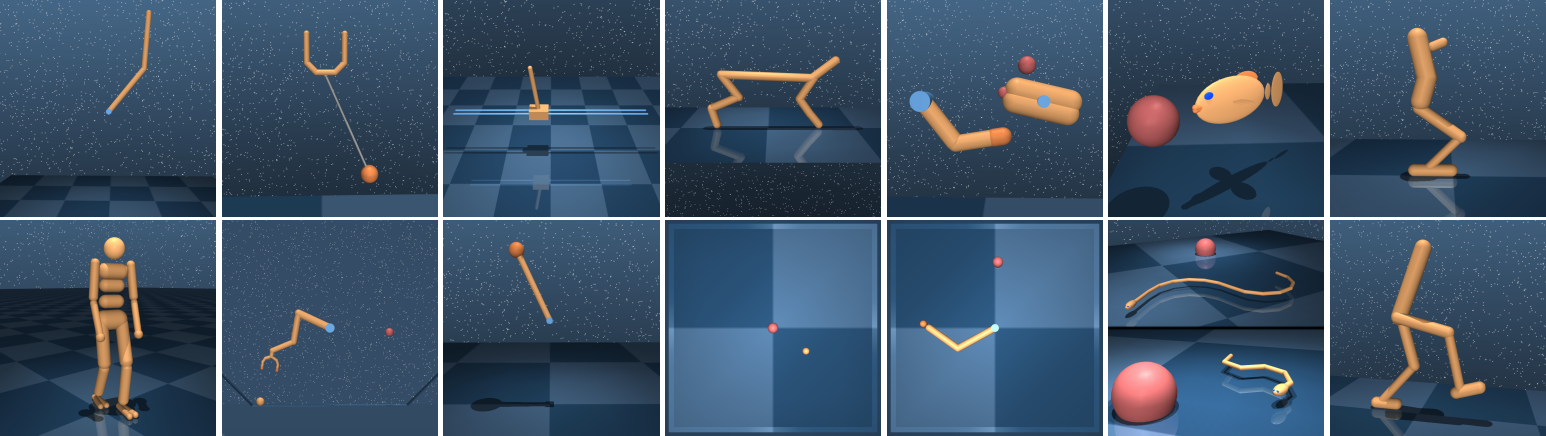
\includegraphics[width=1.0\textwidth]{./chapters/chapter_1/imgs/img_ch1_benchmarks_controlsuite.png}
            \caption{}
            \label{fig:ch1_benchmarks_controlsuite}
        \end{subfigure}
        %% Roboschool
        \centering
        \begin{subfigure}[b]{1.0\textwidth}
            \centering
            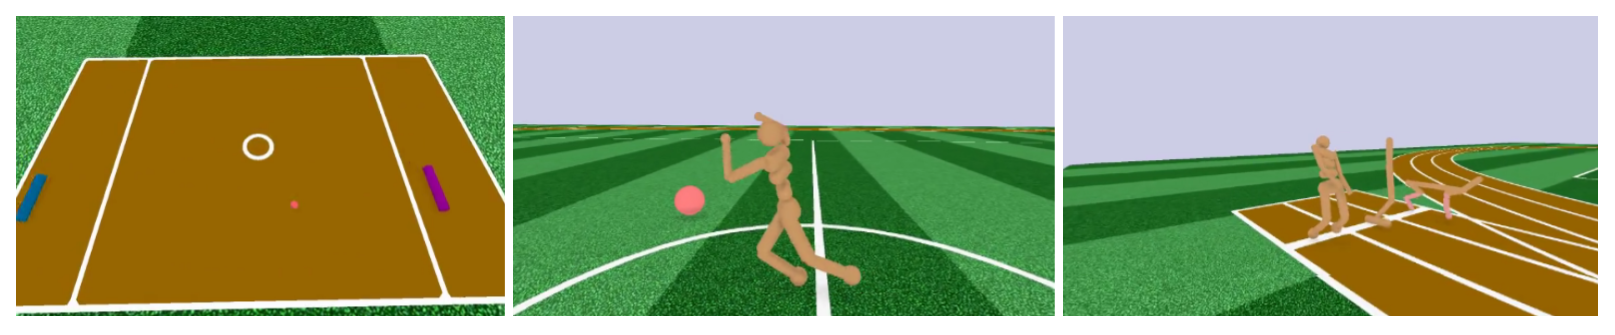
\includegraphics[width=1.0\textwidth]{./chapters/chapter_1/imgs/img_ch1_benchmarks_roboschool.png}
            \caption{}
            \label{fig:ch1_benchmarks_roboschool}
        \end{subfigure}
        %% Gym
        \centering
        \begin{subfigure}[b]{1.0\textwidth}
            \centering
            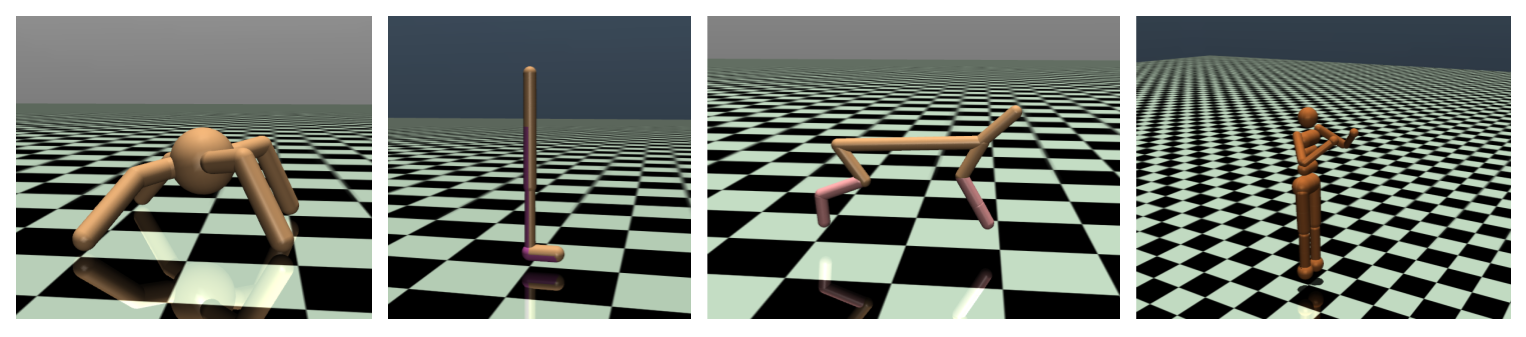
\includegraphics[width=1.0\textwidth]{./chapters/chapter_1/imgs/img_ch1_benchmarks_gym.png}
            \caption{}
            \label{fig:ch1_benchmarks_gym}
        \end{subfigure}
        %% Rllab
        \centering
        \begin{subfigure}[b]{1.0\textwidth}
            \centering
            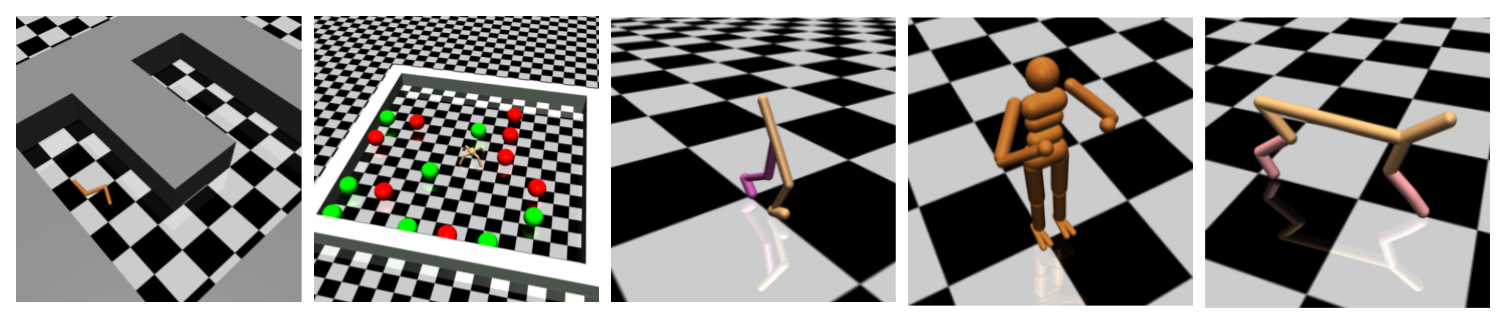
\includegraphics[width=1.0\textwidth]{./chapters/chapter_1/imgs/img_ch1_benchmarks_rllab.png}
            \caption{}
            \label{fig:ch1_benchmarks_rllab}
        \end{subfigure}
        \caption{Available benchmarks for locomotion tasks: 
                            a) controlsuite \citep{Controlsuite},
                            b) roboschool \citep{Roboschool},
                            c) gym \citep{Gym} and
                            d) rllab \citep{Rllab}}
        \label{fig:ch1_drl_locomotion_benchmarks}
    \end{figure}
}

\newcommand{\figEnvironmentsProposalFromTo}{
    \begin{figure}
        \centering
        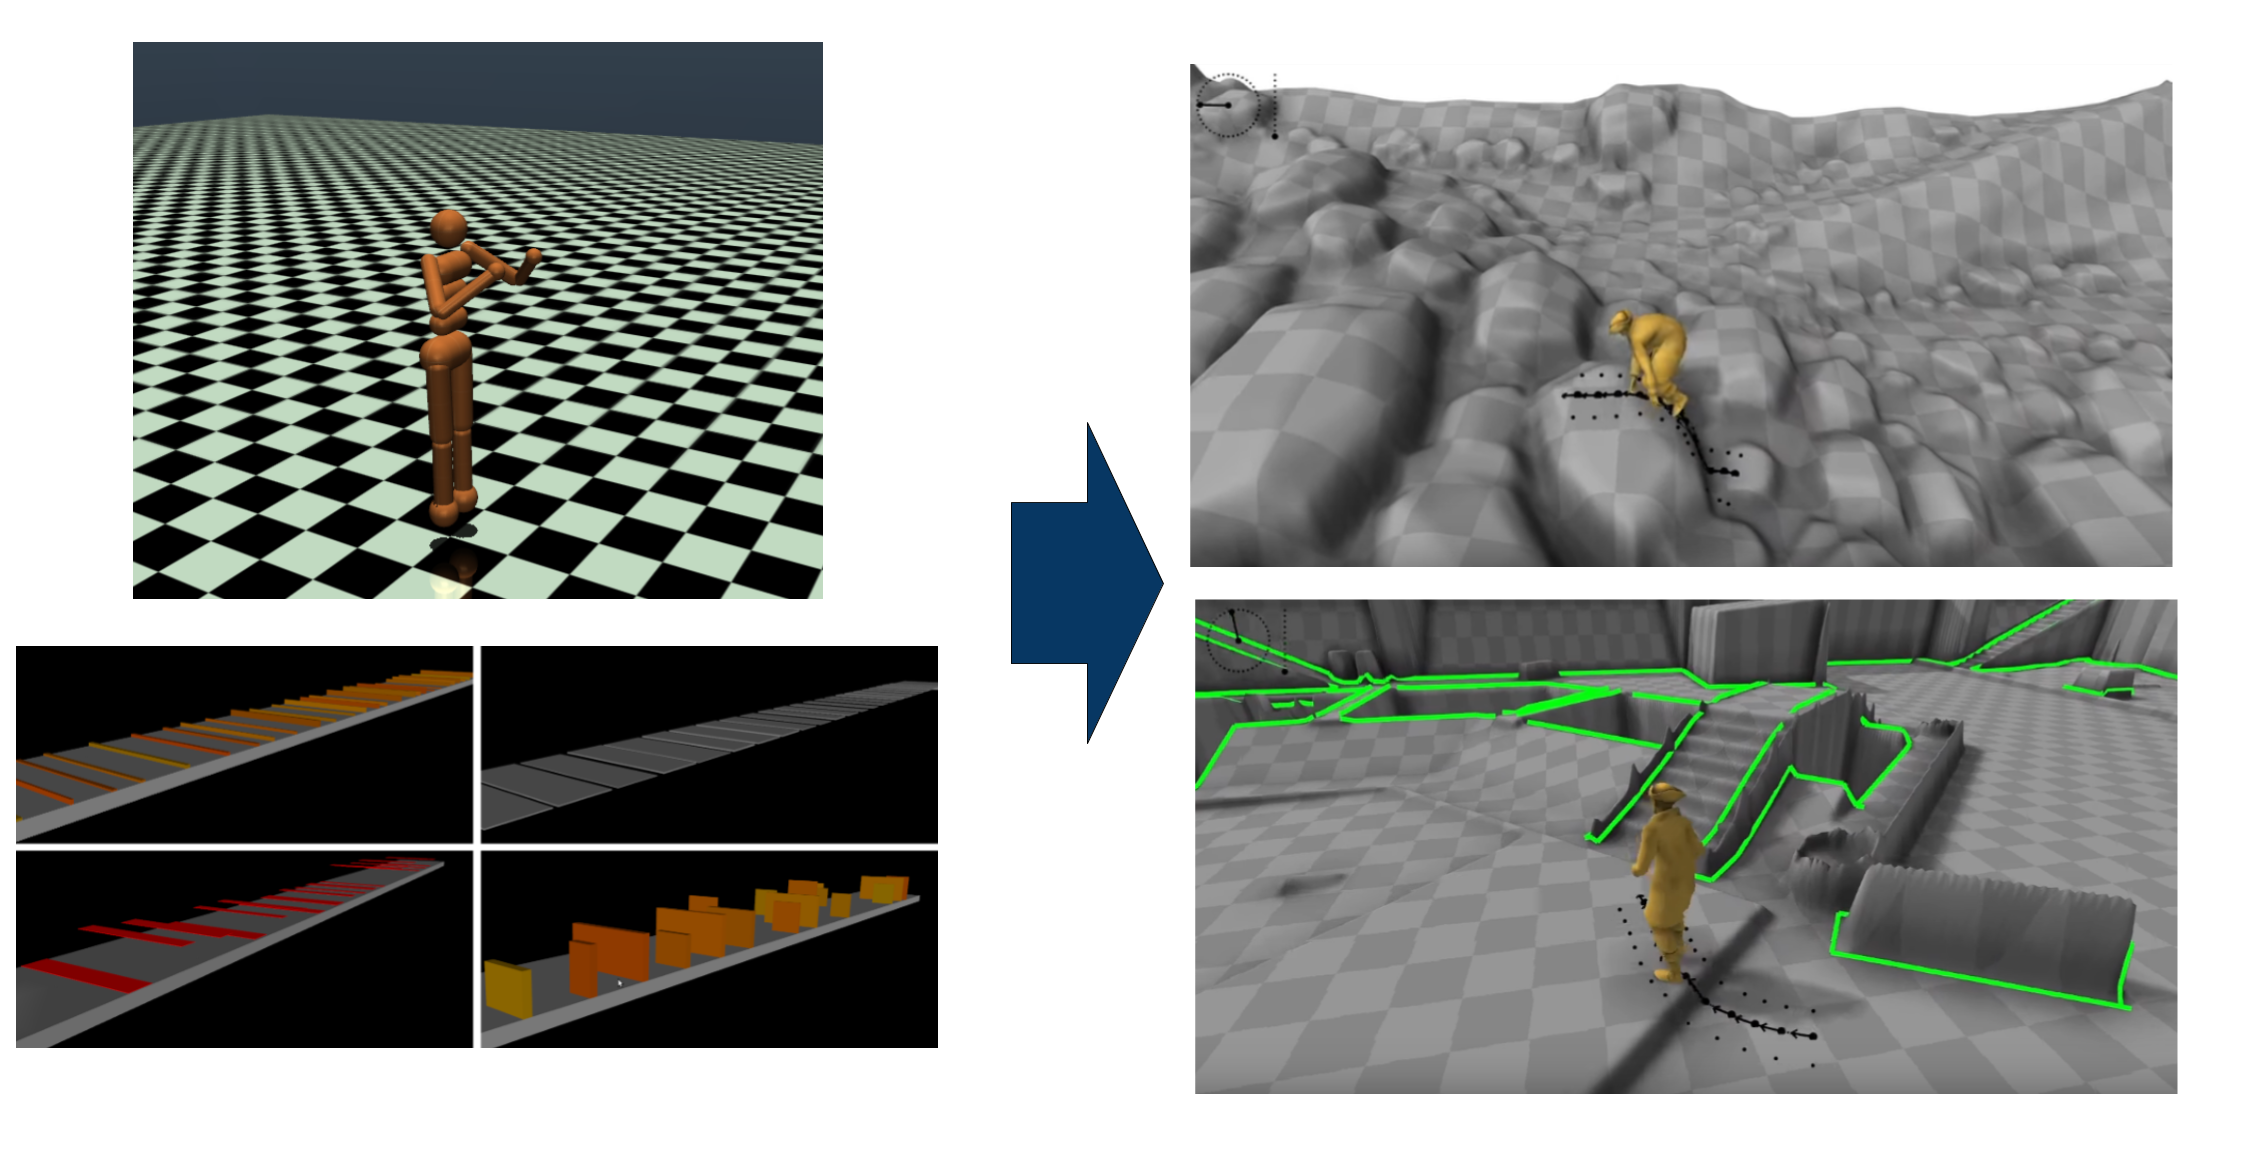
\includegraphics[width=0.8\textwidth]{./chapters/chapter_1/imgs/img_ch1_environments_from_to.png}
        \caption{Comparison of the proposed environments to environments from current benchmarks. 
                 Left: relatively simple environments (image adapted from \citet{Gym}). 
                 Right: relatively more complex proposed environments (images adapted from \citet{Pfnn} ).}
        \label{fig:ch1_environments_comparison_from_to}
    \end{figure}
}

\newcommand{\figEnvManipSimToreal}{
    \begin{figure}
        \centering
        \begin{subfigure}[b]{0.45\textwidth}
            \centering
            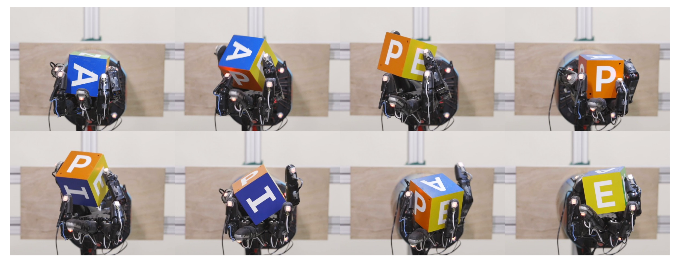
\includegraphics[width=0.9\textwidth]{./chapters/chapter_1/imgs/img_ch1_openai_robot_dexterity.png}
            \caption{}
            \label{fig:ch1_openai_robot_dexterity}
        \end{subfigure}
        \begin{subfigure}[b]{0.45\textwidth}
            \centering
            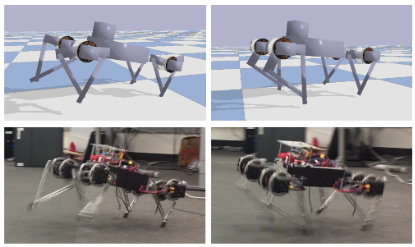
\includegraphics[width=0.9\textwidth]{./chapters/chapter_1/imgs/img_ch1_google_brain_minitaur_sim_to_real.png}
            \caption{}
            \label{fig:ch1_google_brain_minitaur_sim_to_real}
        \end{subfigure}
        \caption{Some examples of sim2real results: 
                            a) Robotic hand generalizing in randomized environment \citep{OpenAISim2real}.
                            b) Quadruped trained in simulation and deployed in real world \citep{GoogleBrainSim2Real} }
        \label{fig:ch1_sim_to_real_approaches}
    \end{figure}
}